\documentclass[12pt]{article}
\usepackage[T1]{fontenc}
\usepackage[utf8]{inputenc}
\usepackage{lmodern}
\usepackage[margin=1.15in]{geometry}
\usepackage{
  amsmath,amssymb,booktabs,threeparttable,microtype,
  setspace,natbib,graphicx,float
}
\usepackage{xcolor,hyperref}
\hypersetup{
  colorlinks=true,
  linkcolor=blue!50!black,
  citecolor=blue!50!black,
  urlcolor=blue!50!black,
  pdftitle={Financing Population Aging: Tax Mix, Public Debt, and Informality in Colombia},
  pdfauthor={Oliver Pardo}
}
\onehalfspacing
\setlength{\emergencystretch}{2em}
\graphicspath{{figures/}}
\newcommand{\dd}{\,\mathrm{d}}
\newcommand{\E}{\mathbb{E}}
\newcommand{\DependencyTwentyTwentyFour}{15.02\%}
\newcommand{\DependencyTwentyFifty}{27.28\%}
\newcommand{\DependencyTwentySeventy}{48.17\%}
\newcommand{\BenchmarkInformality}{55.4\%}
\newcommand{\BenchmarkOutlayShare}{5.7\%}
\newcommand{\OptimalConsumptionShareTwentyTwentyFour}{92.5\%}
\newcommand{\OptimalPayrollShareTwentyTwentyFour}{7.5\%}
\newcommand{\OptimalConsumptionShareTwentyFifty}{82.5\%}
\newcommand{\OptimalPayrollShareTwentyFifty}{17.5\%}
\newcommand{\OptimalConsumptionShareTwentySeventy}{75.0\%}
\newcommand{\OptimalPayrollShareTwentySeventy}{25.0\%}
\newcommand{\OptimalConsumptionTaxTwentyFifty}{17.4\%}
\newcommand{\OptimalPayrollTaxTwentyFifty}{4.5\%}
\newcommand{\OptimalInformalityTwentyFifty}{56.0\%}
\newcommand{\OptimalCapitalTwentyFifty}{2.614}
\newcommand{\FrictionlessConsumptionShare}{100.0\%}


\title{\textbf{Financing Population Aging:}\\
\large Tax Mix, Public Debt, and Informality in Colombia}
\author{
  Oliver Pardo\thanks{
    Departamento de Administraci{\'o}n, Pontificia Universidad Javeriana,
    Bogot{\'a}, Colombia.
    Email: \href{mailto:pardoo@javeriana.edu.co}{pardoo@javeriana.edu.co}.
  }
}
\date{August 2026}

\begin{document}
\maketitle

\begin{abstract}\small\sloppy
\noindent
Population aging raises social-security spending even when the real benefit
or service received by each older adult remains constant. This paper asks how
that permanent fiscal pressure should be distributed across consumption,
formal payroll, and capital-income taxes in an economy with a large informal
sector. I build a stationary general-equilibrium model with formal capital,
labor-intensive informal production, imperfect substitution between formal
and informal consumption goods, endogenous labor informality, public debt,
and convex tax-collection costs. DANE projections raise the ratio of people
aged 65 and over to the population aged 15--64 from
\DependencyTwentyTwentyFour{} in 2024 to \DependencyTwentyFifty{} in 2050
and \DependencyTwentySeventy{} in 2070. At Colombia's statutory debt anchor
of 55 percent of GDP, the model assigns \OptimalConsumptionShareTwentyFifty{}
of the 2050 revenue requirement to consumption and
\OptimalPayrollShareTwentyFifty{} to payroll; the stationary capital-income
tax is zero. The associated effective rates are
\OptimalConsumptionTaxTwentyFifty{} and \OptimalPayrollTaxTwentyFifty{},
and informality is \OptimalInformalityTwentyFifty{}. As aging intensifies,
the payroll share rises because concentrating revenue in a single base has a
convex resource cost. Without that collection friction, the model returns the
corner solution of \FrictionlessConsumptionShare{} consumption taxation.
Raising the debt anchor does not finance aging in the long run: it increases
the stationary interest bill and required revenue. These numerical shares are
mechanism results, not a tax proposal. The benchmark has one representative
household and provisional collection costs; it therefore excludes
distributional incidence, intragenerational consumption variance, and a
perfect-foresight transition.

\medskip\noindent
\textbf{Keywords:} population aging; optimal tax mix; public debt;
informality; Colombia.
\quad
\textbf{JEL:} E62; H21; H55; H63; J46.
\end{abstract}\fussy

\section{Introduction}

Population aging changes the fiscal problem even if social-security rules do
not change. Suppose that every older adult receives a fixed real amount of
pensions, health services, or long-term care. The government's outlay per
working-age adult then rises with the ratio of older people to the population
that supplies most labor and pays most taxes. Debt can postpone part of the
adjustment. It cannot replace the permanent revenue that a permanently older
population requires.

This paper asks which combination of consumption, formal-payroll, and
capital-income taxes finances that pressure at the lowest stationary welfare
cost. The question is particularly relevant for Colombia because the tax
bases are not equally broad. A payroll tax applies directly to formal
employment. A consumption tax reaches formal purchases and only part of
informal transactions. A capital-income tax falls on the input used by the
formal sector but not by the labor-intensive informal sector. Each instrument
therefore changes both the revenue collected from its own base and the
allocation of labor and capital between sectors.

The demographic input comes directly from DANE's 2025 national population
projections. Let $N_t^o$ denote the population aged 65 and over and $N_t^y$
the population aged 15--64. DANE projects that
\[
 d_t=\frac{N_t^o}{N_t^y}
\]
rises from \DependencyTwentyTwentyFour{} in 2024 to
\DependencyTwentyFifty{} in 2050 and \DependencyTwentySeventy{} in 2070
\citep{DANE2025Projections}. If the real outlay per older adult is
$\bar g_o$, social-security spending per working-age adult is the identity
\[
 G_t^{SS}=\bar g_o d_t.
\]
This formulation turns population aging into a fiscal requirement without
assuming an arbitrary expenditure shock.

The model adds four margins to that identity. First, formal and informal
consumption goods enter a constant-elasticity-of-substitution aggregator.
They are substitutes, but not perfect substitutes. Second, only formal
production uses capital. Third, workers choose formal or informal employment
according to after-tax relative wages and heterogeneous sector preferences.
Fourth, raising a tax has a convex real collection cost that represents
administration, compliance, and resources lost through avoidance and
enforcement. This last margin matters for the tax mix: without it, spreading
revenue across bases has no direct benefit.

Public debt enters through the government's flow budget and a fiscal reaction
rule. The benchmark uses the 55-percent-of-GDP net-debt anchor established by
Law 2155 of 2021; the same law defines a 71-percent limit
\citep{Law2155}. The model varies the anchor between 40 and 70 percent to show
how $\bar q$ changes the stationary interest bill. This is a long-run
comparative static. It does not quantify the possible gain from issuing debt
during the demographic transition and repaying it later.

The calibration matches \BenchmarkInformality{} labor informality and
normalizes initial public pension spending to \BenchmarkOutlayShare{} of GDP,
the value reported for Colombia by the OECD
\citep{DANE2025Informality,OECD2023Colombia}. The remaining parameters,
including the collection-cost coefficient and the fraction of
social-security spending that purchases real goods and services, are
provisional. The numerical exercise should therefore be read as a disciplined
mechanism comparison.

Three results organize the paper. First, the frictionless benchmark produces
a corner: all revenue is raised from consumption. A CES distinction between
formal and informal goods does not by itself generate an interior tax mix.
Second, common convex collection costs produce a combination of consumption
and payroll taxes. At the 55-percent debt anchor, the consumption share falls
from \OptimalConsumptionShareTwentyTwentyFour{} in 2024 to
\OptimalConsumptionShareTwentyFifty{} in 2050 and
\OptimalConsumptionShareTwentySeventy{} in 2070. The payroll share rises
correspondingly. The stationary capital-income tax remains zero because this
representative-household model contains neither a distributional motive nor
capital rents. Third, a higher debt anchor raises long-run required revenue.
Moving the anchor from 40 to 70 percent of GDP lowers stationary composite
consumption by about 0.6 percent in the 2050 demographic equilibrium.

The next section relates the exercise to the literature. Section 3 presents
the model. Section 4 describes the calibration and the numerical policy
experiment. Section 5 reports the results. Section 6 states the limitations
that restrict their policy interpretation. The appendix describes the
algorithm.

\section{Related literature}

The paper connects three bodies of work. The first is the optimal-tax
literature. \citet{DiamondMirrlees1971a,DiamondMirrlees1971b} characterize
efficient production and tax rules when the government must raise revenue
with distortionary instruments. The long-run capital-tax result in
\citet{Chamley1986} shows why a tax on the return to an accumulated factor can
have a large stationary cost. The present model is narrower than those
general results. It compares three proportional tax bases in a quantitative
two-sector economy and introduces collection costs directly in the resource
constraint.

The second body of work studies taxation when part of economic activity is
informal. \citet{EmranStiglitz2005} show that incomplete value-added-tax
coverage changes standard indirect-tax prescriptions.
\citet{GordonLi2009} explain several features of developing-country tax
systems through firms' ability to avoid taxes outside the financial system.
\citet{Keen2007} emphasizes that a value-added tax can still reach informal
operators through taxed formal inputs and imports. This paper captures that
partial reach with a parameter that applies the consumption tax to a fraction
of informal expenditure.

Informality is an equilibrium allocation, not a fixed untaxed base.
\citet{LaPortaShleifer2014} review its relationship with development.
\citet{Ulyssea2018} models firms' extensive and intensive formalization
decisions. For Colombia, \citet{Osorio2016} and
\citet{GrandaMorales2023} study how tax policy and labor-market rigidities
affect informality. The present paper uses a smooth labor-regime choice. The
purpose is not to reproduce every margin of firm informality, but to preserve
the feedback from a formal-payroll tax to the number of formal workers and
therefore to its own revenue base.

The third body of work concerns public debt. In the tax-smoothing argument of
\citet{Barro1979}, debt can distribute temporary fiscal pressures across
time when the excess burden of taxation is convex. \citet{Bohn1998} studies
the positive response of primary surpluses to debt as a condition for fiscal
sustainability. The fiscal rule used below combines both ideas: debt evolves
through the government budget, and the primary surplus responds positively
when debt lies above its anchor. The aging shock is permanent, however. Debt
can smooth its arrival but cannot eliminate its present-value tax cost.

Finally, the Colombian pension literature documents the size and fiscal risks
of the existing system \citep{Ospina2024}. This paper does not model a
specific pension regime. It studies the financing problem created by any
old-age outlay that remains fixed per beneficiary while the number of
beneficiaries rises relative to the working-age population.

\section{Model}

\subsection{Population aging and social-security spending}

The economy is normalized by the working-age population. The old-age
dependency ratio is $d_t=N_t^o/N_t^y$. A fixed real outlay $\bar g_o$ per older
adult implies
\begin{equation}
  G_t^{SS}=\bar g_o d_t.
  \label{eq:social_spending}
\end{equation}
Social-security outlays combine transfers and real public services. Let
$\zeta\in[0,1]$ denote the share that purchases health, care, administration,
or other real resources:
\begin{equation}
  G_t^R=\zeta G_t^{SS},
  \qquad
  T_t^o=(1-\zeta)G_t^{SS}.
  \label{eq:resource_transfer_split}
\end{equation}
Transfers redistribute purchasing power inside the representative dynasty.
Only $G_t^R$ absorbs goods in the aggregate resource constraint. This
distinction prevents a pension payment from being treated mechanically as if
the transferred resources disappeared.

\subsection{Household, consumption, and asset accumulation}

The representative dynasty maximizes
\begin{equation}
  \sum_{t=0}^{\infty}\beta^t
  \left[
    \frac{C_t^{1-\sigma}-1}{1-\sigma}
    +\chi_G\log G_t^R
  \right].
  \label{eq:utility}
\end{equation}
The benchmark sets $\chi_G=0$. It therefore asks which tax mix preserves
private consumption, not whether additional social-security services produce
benefits.

Formal and informal consumption are imperfect substitutes:
\begin{equation}
 C_t=
 \left[
   \varpi^{1/\eta}(C_t^F)^{(\eta-1)/\eta}
   +(1-\varpi)^{1/\eta}(C_t^I)^{(\eta-1)/\eta}
 \right]^{\eta/(\eta-1)},
 \label{eq:ces}
\end{equation}
where $\eta$ is the elasticity of substitution and $\varpi$ is the formal-good
weight. The formal producer price is normalized to one. The consumer prices
are
\begin{equation}
 \widetilde p_t^F=1+\tau_t^c,
 \qquad
 \widetilde p_t^I=p_t^I(1+\xi_I\tau_t^c),
 \label{eq:consumer_prices}
\end{equation}
where $\xi_I\in[0,1]$ is the fraction of informal expenditure reached
indirectly by the consumption tax. The CES price index and relative demand
are
\begin{align}
 P_t^C
 &=
 \left[
   \varpi(\widetilde p_t^F)^{1-\eta}
   +(1-\varpi)(\widetilde p_t^I)^{1-\eta}
 \right]^{1/(1-\eta)},                                      \label{eq:price_index}\\
 \frac{C_t^F}{C_t^I}
 &=
 \frac{\varpi}{1-\varpi}
 \left(\frac{\widetilde p_t^F}{\widetilde p_t^I}\right)^{-\eta}.
 \label{eq:relative_demand}
\end{align}

The household holds productive capital and government bonds. Its consolidated
budget can be written as
\begin{align}
 P_t^C C_t+K_{t+1}+B_{t+1}
 &=(1-\tau_t^p)w_t^F L_t^F+w_t^I L_t^I \nonumber\\
 &\quad+
 \left[1-\delta+(1-\tau_t^k)r_t^K\right]K_t
 +(1+r_t^b)B_t+T_t^o.
 \label{eq:household_budget}
\end{align}
The steady-state Euler conditions for two assets held in positive amounts are
\begin{equation}
  1=\beta\left[1-\delta+(1-\tau^k)r^K\right]
   =\beta(1+r^b).
  \label{eq:euler}
\end{equation}
The calibration sets $\beta=1/(1+r^b)$, so the stationary bond and capital
returns are consistent.

\subsection{Formal and informal production}

Formal firms use capital and formal labor:
\begin{equation}
  Y_t^F=A_FK_t^\alpha(L_t^F)^{1-\alpha}.
  \label{eq:formal_production}
\end{equation}
Competitive factor prices are
\begin{equation}
  w_t^F=(1-\alpha)\frac{Y_t^F}{L_t^F},
  \qquad
  r_t^K=\alpha\frac{Y_t^F}{K_t}.
  \label{eq:factor_prices}
\end{equation}
Informal production is labor intensive:
\begin{equation}
  Y_t^I=A_I L_t^I,
  \qquad
  w_t^I=p_t^I A_I.
  \label{eq:informal_production}
\end{equation}
Labor satisfies $L_t^F+L_t^I=1$. The assumption that only formal production
uses capital gives payroll and capital taxation a common formal-sector base,
while preserving different intensive margins.

\subsection{Endogenous labor informality}

Workers receive idiosyncratic preferences for the two labor regimes. With a
logistic difference in those preferences, the formal share is
\begin{equation}
  L_t^F=
  \Lambda\left(
    \frac{
      \log[(1-\tau_t^p)w_t^F]-\log(w_t^I)-\kappa
    }{\mu}
  \right),
  \qquad
  \Lambda(x)=\frac{1}{1+e^{-x}}.
  \label{eq:formal_choice}
\end{equation}
The fixed cost $\kappa$ shifts the average return to formal employment and
$\mu$ controls the dispersion of regime preferences. For finite $\mu$, both
labor regimes coexist. A payroll tax lowers the net formal wage and increases
informality. A consumption tax affects informality indirectly through the
relative demand for formal and informal goods.

\subsection{Government revenue, debt, and the fiscal rule}

The government raises revenue from consumption, formal payroll, and capital
income:
\begin{align}
 R_t^c&=\tau_t^c
   \left(C_t^F+\xi_Ip_t^IC_t^I\right),                       \label{eq:revenue_c}\\
 R_t^p&=\tau_t^p w_t^F L_t^F,                               \label{eq:revenue_p}\\
 R_t^k&=\tau_t^k r_t^K K_t,                                 \label{eq:revenue_k}\\
 R_t&=R_t^c+R_t^p+R_t^k.                                    \label{eq:revenue_total}
\end{align}
Debt follows
\begin{equation}
 B_{t+1}=(1+r_t^b)B_t+G_t^{SS}-R_t.
 \label{eq:government_budget}
\end{equation}
Let $q_t=B_t/Y_t^N$, where nominal output is
$Y_t^N=Y_t^F+p_t^IY_t^I$. If trend output grows at rate $\gamma$, the primary
surplus ratio that stabilizes debt at $q$ is $(r^b-\gamma)q$. The fiscal
reaction function is
\begin{equation}
 \frac{R_t-G_t^{SS}}{Y_t^N}
 =
 (r_t^b-\gamma)q_t
 +\phi_q(q_t-\bar q).
 \label{eq:fiscal_rule}
\end{equation}
The feedback coefficient $\phi_q>0$ raises the surplus when debt exceeds the
anchor. In the stationary experiments $q=\bar q$, so the second term is zero.

\subsection{Collection costs and market clearing}

Collecting a higher rate from a given base uses real resources. The reduced
form is
\begin{equation}
 \Psi_t=
 \frac{1}{2}\sum_{j\in\{c,p,k\}}
 \chi_j(\tau_t^j)^2\mathcal B_t^j,
 \label{eq:collection_cost}
\end{equation}
where $\mathcal B_t^j$ is the corresponding base in
equations \eqref{eq:revenue_c}--\eqref{eq:revenue_k}. The term includes tax
administration, private compliance, enforcement, and avoidance resources. It
does not represent revenue lost to the government; it is a real cost in the
formal-goods market.

Capital accumulation and goods-market clearing are
\begin{align}
 K_{t+1}&=(1-\delta)K_t+I_t,                                 \label{eq:capital_law}\\
 Y_t^F&=C_t^F+I_t+G_t^R+\Psi_t,                              \label{eq:formal_market}\\
 Y_t^I&=C_t^I.                                               \label{eq:informal_market}
\end{align}
At a stationary equilibrium, $I=\delta K$. Pension transfers do not enter
equation \eqref{eq:formal_market}; their recipients use them to purchase the
goods already included in private consumption.

\subsection{Tax mix and policy problem}

Let $\boldsymbol{\omega}=(\omega_c,\omega_p,\omega_k)$ denote the shares of
required revenue assigned to the three bases:
\begin{equation}
  R^j=\omega_jR,
  \qquad
  \omega_c+\omega_p+\omega_k=1,
  \qquad
  \omega_j\geq0.
  \label{eq:tax_shares}
\end{equation}
Given an equilibrium allocation, tax rates satisfy
\begin{equation}
  \tau^j=\frac{\omega_jR}{\mathcal B^j}.
  \label{eq:tax_rates}
\end{equation}
For each dependency ratio and debt anchor, the stationary Ramsey problem is
\begin{equation}
 \max_{\boldsymbol{\omega}\in\Delta^2}
 \frac{u(C(\boldsymbol{\omega}))}{1-\beta}
 \quad
 \text{subject to equations \eqref{eq:social_spending}--\eqref{eq:tax_rates}.}
 \label{eq:ramsey_problem}
\end{equation}
Because $u(C)$ is increasing and $\chi_G=0$, this is equivalent to maximizing
stationary composite consumption. The tax mix is chosen on a simplex; the
model does not impose an interior solution.

\section{Calibration and numerical experiment}

Table \ref{tab:calibration} reports the benchmark calibration. Formal
production uses a capital share of 0.33 and annual depreciation of 0.06. A
four-percent real bond rate implies $\beta=1/1.04$. The CES elasticity is 1.5:
formal and informal goods are substitutes, but far from perfect substitutes.
The consumption tax reaches 15 percent of informal expenditure.

\begin{table}[H]
\centering
\caption{Benchmark calibration}
\label{tab:calibration}
\begin{threeparttable}
\begin{tabular}{llrl}
\toprule
Parameter & Symbol & Value & Status \\
\midrule
Formal capital share & $\alpha$ & 0.330 & Provisional \\
Annual depreciation & $\delta$ & 0.060 & Provisional \\
Annual discount factor & $\beta$ & 0.962 & Implied by $r^b$ \\
CES elasticity & $\eta$ & 1.500 & Provisional \\
Informal VAT coverage & $\xi_I$ & 0.150 & Provisional \\
Regime-choice scale & $\mu$ & 0.300 & Provisional \\
Outlay per older adult & $\bar g_o$ & 0.426 & Calibrated \\
Formal-work fixed cost & $\kappa$ & 0.633 & Calibrated \\
Real-resource share & $\zeta$ & 0.250 & Provisional \\
Real bond rate & $r^b$ & 0.040 & Provisional \\
Trend output growth & $\gamma$ & 0.010 & Provisional \\
Debt anchor & $\bar q$ & 0.550 & Law 2155 of 2021 \\
Common collection cost & $\chi_j$ & 2.000 & Provisional \\
\bottomrule
\end{tabular}
\begin{tablenotes}\footnotesize
\item Notes: The calibration uses a reference revenue mix of 45 percent
consumption, 35 percent payroll, and 20 percent capital income.
$\bar g_o$ matches public pension spending of 5.7 percent of GDP, and
$\kappa$ matches 55.4 percent labor informality. Effective tax rates and model
units should not be read as statutory Colombian rates.
\end{tablenotes}
\end{threeparttable}
\end{table}

Two parameters match Colombian targets under the reference revenue mix.
$\bar g_o$ matches public pension spending of \BenchmarkOutlayShare{} of GDP
\citep{OECD2023Colombia}. $\kappa$ matches \BenchmarkInformality{} national
labor informality \citep{DANE2025Informality}. The reference mix is a
normalization, not an estimate of the composition of Colombian tax revenue.

The debt anchor is 55 percent of GDP. Law 2155 defines that value for net debt
of the central government and a 71-percent limit \citep{Law2155}. The
counterfactuals use anchors of 40, 55, and 70 percent. They keep the structural
parameters and $\bar g_o$ fixed.

The demographic experiment reads every annual value between 2024 and 2070
from DANE's national projections \citep{DANE2025Projections}. For each year,
the code solves a stationary equilibrium conditional on that year's $d_t$.
The resulting annual line is a sequence of conditional steady states. It is
not a perfect-foresight transition with predetermined capital and debt.

The collection-cost coefficients are equal across instruments. This choice
does not favor one base by assigning it a lower primitive collection cost.
Their common level is not empirically estimated. I therefore report the
frictionless case $\chi_j=0$ to identify which conclusion depends on convex
collection costs.

\section{Results}

\subsection{The stationary tax mix}

Table \ref{tab:optimal_mix} reports the tax mix that maximizes stationary
composite consumption at three points on the DANE demographic path. All
shares and rates are percentages. In 2024, the model assigns
\OptimalConsumptionShareTwentyTwentyFour{} of required revenue to
consumption and \OptimalPayrollShareTwentyTwentyFour{} to formal payroll. In
2050, the shares are \OptimalConsumptionShareTwentyFifty{} and
\OptimalPayrollShareTwentyFifty{}. By 2070, the payroll share reaches
\OptimalPayrollShareTwentySeventy{}.

\begin{table}[H]
\centering
\caption{Stationary optimal tax mix along the demographic path}
\label{tab:optimal_mix}
\begin{tabular}{lrrrrrr}
\toprule
Year & $\omega_c$ & $\omega_p$ & $\omega_k$ & $\tau_c$ & $\tau_p$ & Informality \\
\midrule
2024 & 92.5 & 7.5 & 0.0 & 11.3 & 1.1 & 54.7 \\
2050 & 82.5 & 17.5 & 0.0 & 17.4 & 4.5 & 56.0 \\
2070 & 75.0 & 25.0 & 0.0 & 30.4 & 11.1 & 58.0 \\
\bottomrule
\end{tabular}

\begin{minipage}{0.88\textwidth}
\footnotesize
\emph{Notes:} $\omega_j$ is the share of required revenue assigned to tax
$j$; $\tau_j$ is the corresponding effective rate. Every entry other than
the year is a percentage. The debt anchor is 55 percent of GDP.
\end{minipage}
\end{table}

The capital-income share is zero in all three stationary optima. The result
has a precise model interpretation. Capital is used only in formal production,
and taxing its return lowers the stationary capital stock through the Euler
condition. The representative household eliminates any redistributive reason
to tax capital, and formal firms earn no rents. The zero result is therefore
consistent with this specification. It is not a general recommendation to
eliminate capital taxation in Colombia.

The payroll share rises as aging increases because collection costs are
convex. Concentrating an ever larger revenue requirement in consumption
raises the marginal resource cost of that instrument. A moderate payroll tax
then costs less than the additional collection resources required by a still
higher consumption rate, despite the payroll tax's direct effect on
informality.

Figure \ref{fig:simplex} shows the 2050 policy search. Each point is a feasible
revenue mix. The lower-left vertex assigns all revenue to consumption, the
lower-right vertex assigns all revenue to payroll, and the top vertex assigns
all revenue to capital income. Darker points have larger
consumption-equivalent losses, capped at eight percent for the color scale.
The star marks the optimum at 82.5 percent consumption and 17.5 percent
payroll. Moving toward the capital vertex lowers consumption sharply.

\begin{figure}[H]
\centering
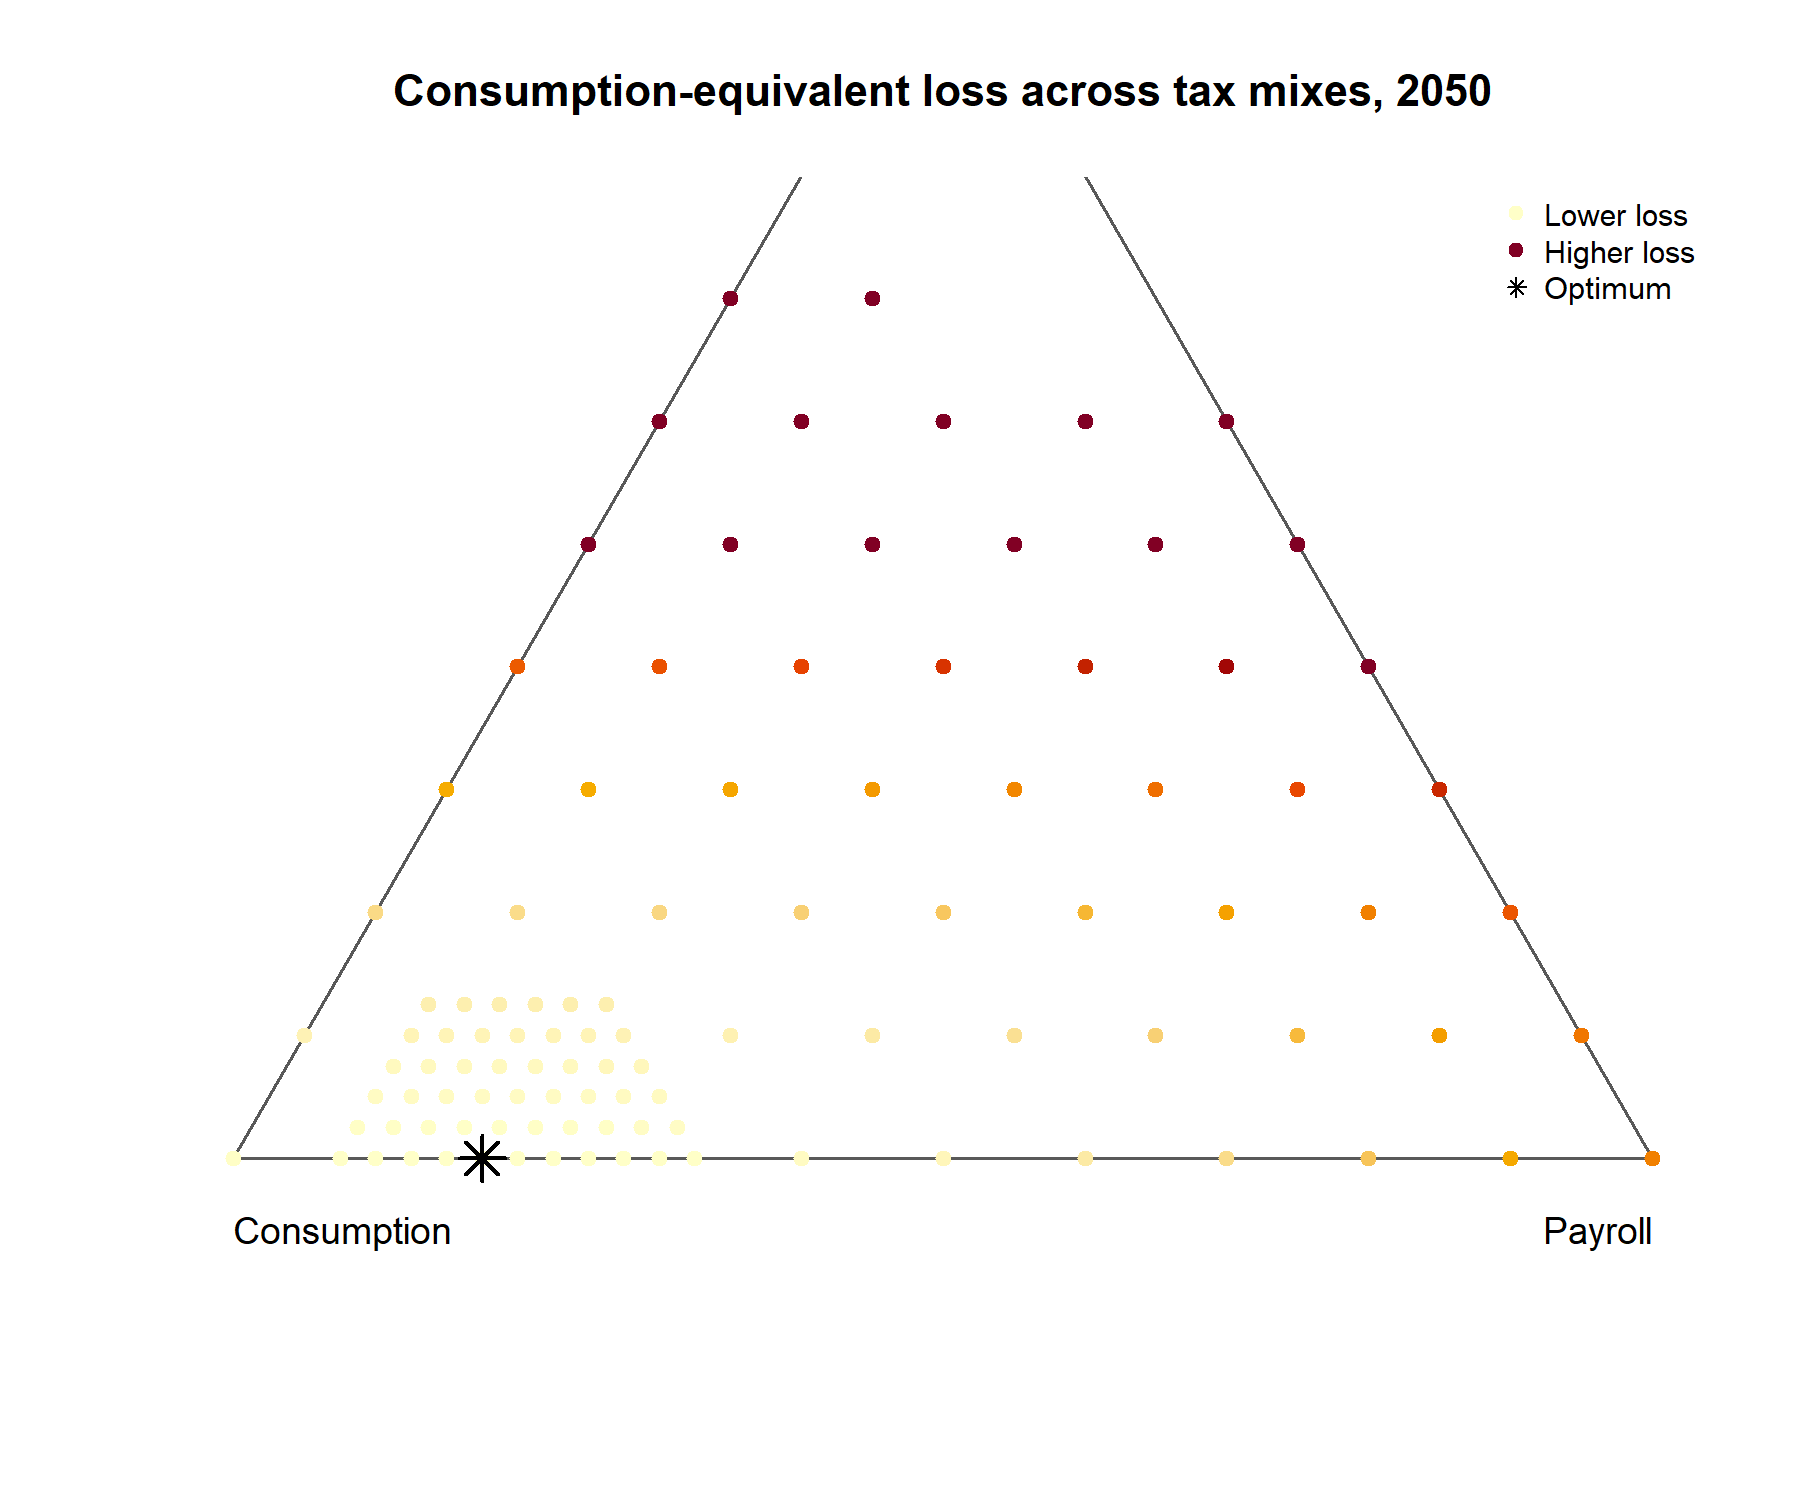
\includegraphics[width=0.82\textwidth]{tax_simplex_2050.png}
\caption{Consumption-equivalent loss across tax mixes in 2050}
\label{fig:simplex}
\begin{minipage}{0.88\textwidth}
\footnotesize
\emph{Notes:} The triangle contains the feasible coarse grid and the local
refinement. Losses are measured relative to the best stationary composite
consumption in the grid. The color scale is capped at eight percent.
\end{minipage}
\end{figure}

Figure \ref{fig:horizons} separates revenue shares from rates. The left panel
shows the shift from consumption toward payroll as $d_t$ rises. The right
panel shows that the effective consumption rate rises from 11.3 percent in
2024 to 17.4 percent in 2050 and 30.4 percent in 2070. The payroll rate rises
from 1.1 to 4.5 and 11.1 percent. The 2070 rates are not a forecast. They show
the pressure created by holding the outlay per older adult fixed while the
dependency ratio more than triples relative to its 2024 level.

\begin{figure}[H]
\centering
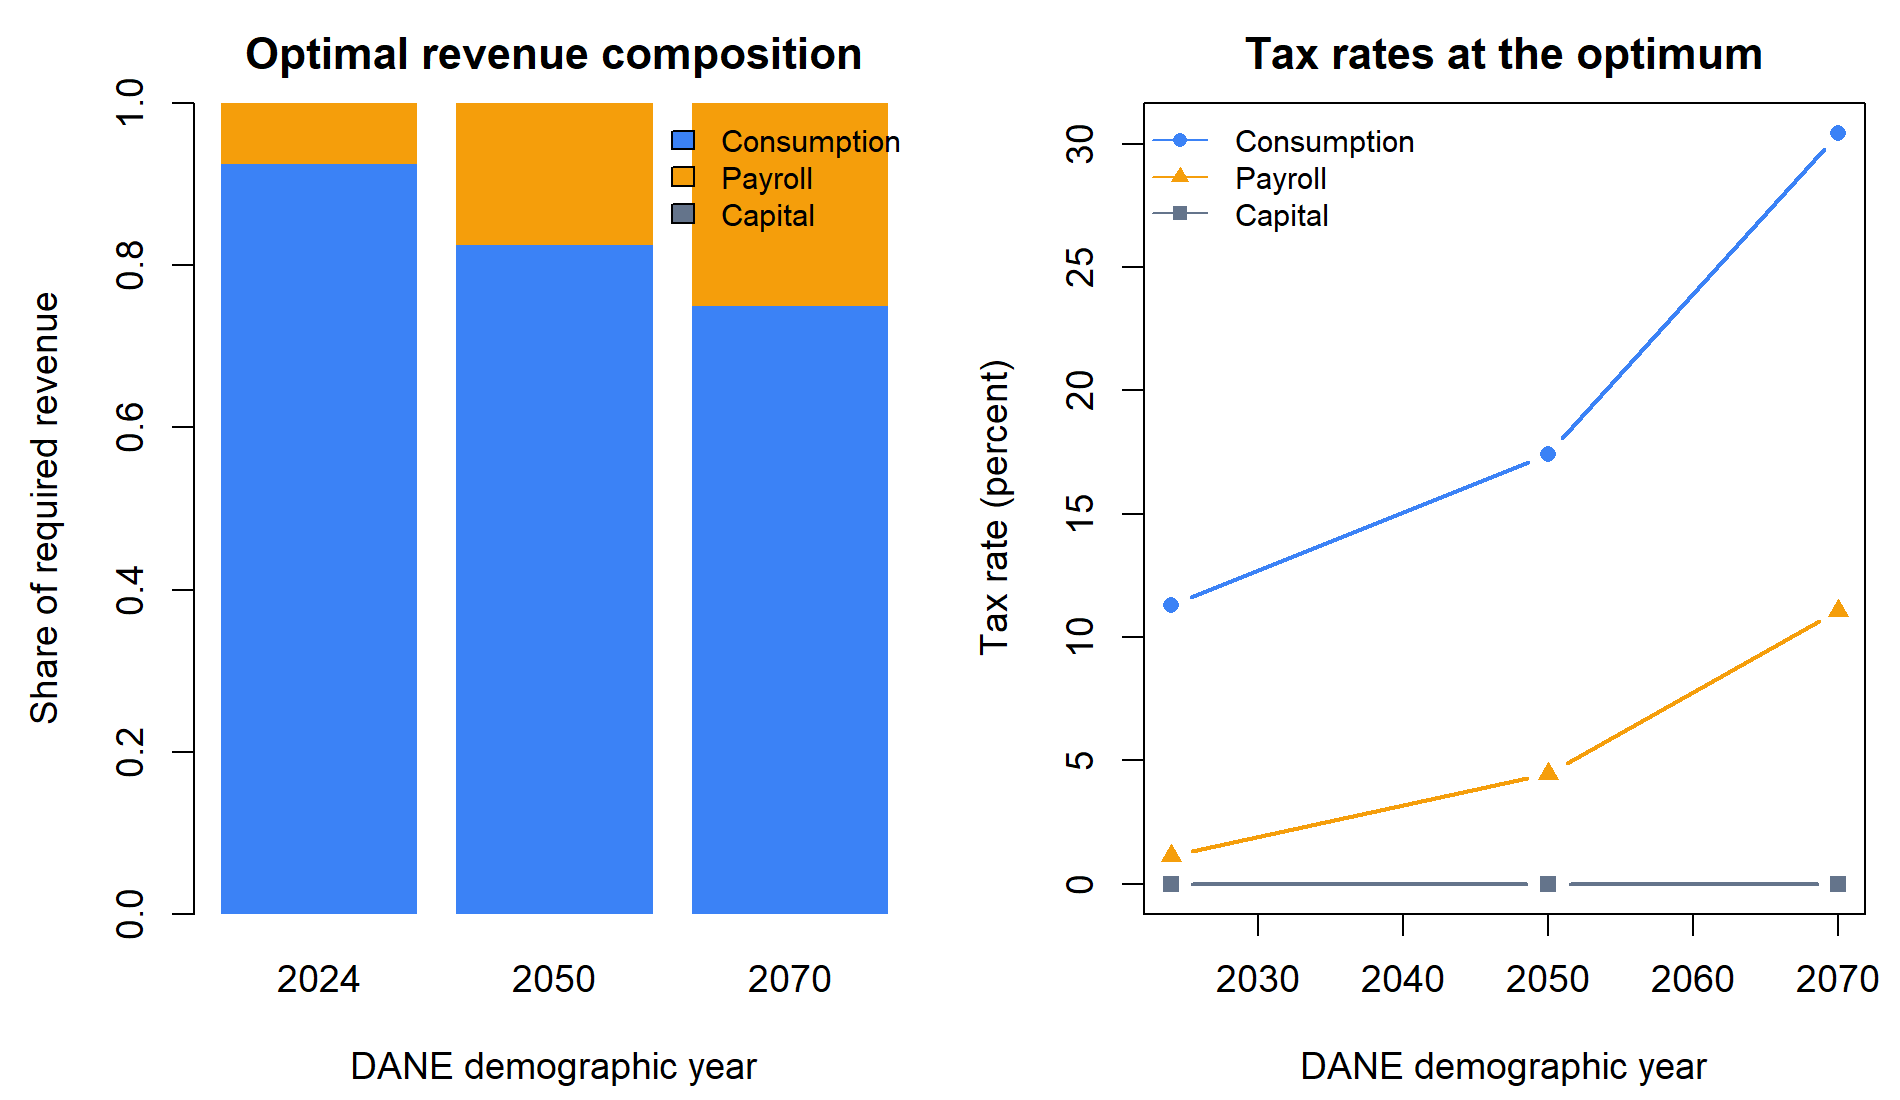
\includegraphics[width=\textwidth]{optimal_mix_horizons.png}
\caption{Optimal revenue composition and effective tax rates}
\label{fig:horizons}
\end{figure}

\subsection{What generates an interior mix?}

The imperfect substitution between formal and informal goods changes the
incidence of the consumption tax. A higher $\tau^c$ raises the relative price
of formal consumption and shifts expenditure toward the informal good. That
mechanism erodes the formal base and changes labor demand. It does not,
however, produce an interior optimum in this calibration.

When all three collection-cost coefficients are set to zero, the 2050 optimum
assigns \FrictionlessConsumptionShare{} of revenue to consumption. Payroll and
capital taxes are both zero. This comparison identifies the source of the
benchmark mix: the CES demand system creates an informal-consumption response,
but convex collection costs create the gain from spreading revenue across
bases.

This result also identifies the paper's main calibration requirement. The
level and instrument-specific values of $\chi_j$ must be estimated before the
numerical shares can support a policy recommendation. The current common
coefficient provides a transparent benchmark, not empirical identification.

\subsection{Conditional demographic paths}

Figure \ref{fig:paths} compares the reference revenue mix with the 2024-optimal
mix held fixed through 2070. The upper-left panel reports social-security
outlays and required revenue under the reference mix. The upper-right panel
reports the three effective rates under the fixed 2024-optimal mix. The lower
panels compare informality and the stationary capital stock.

\begin{figure}[H]
\centering
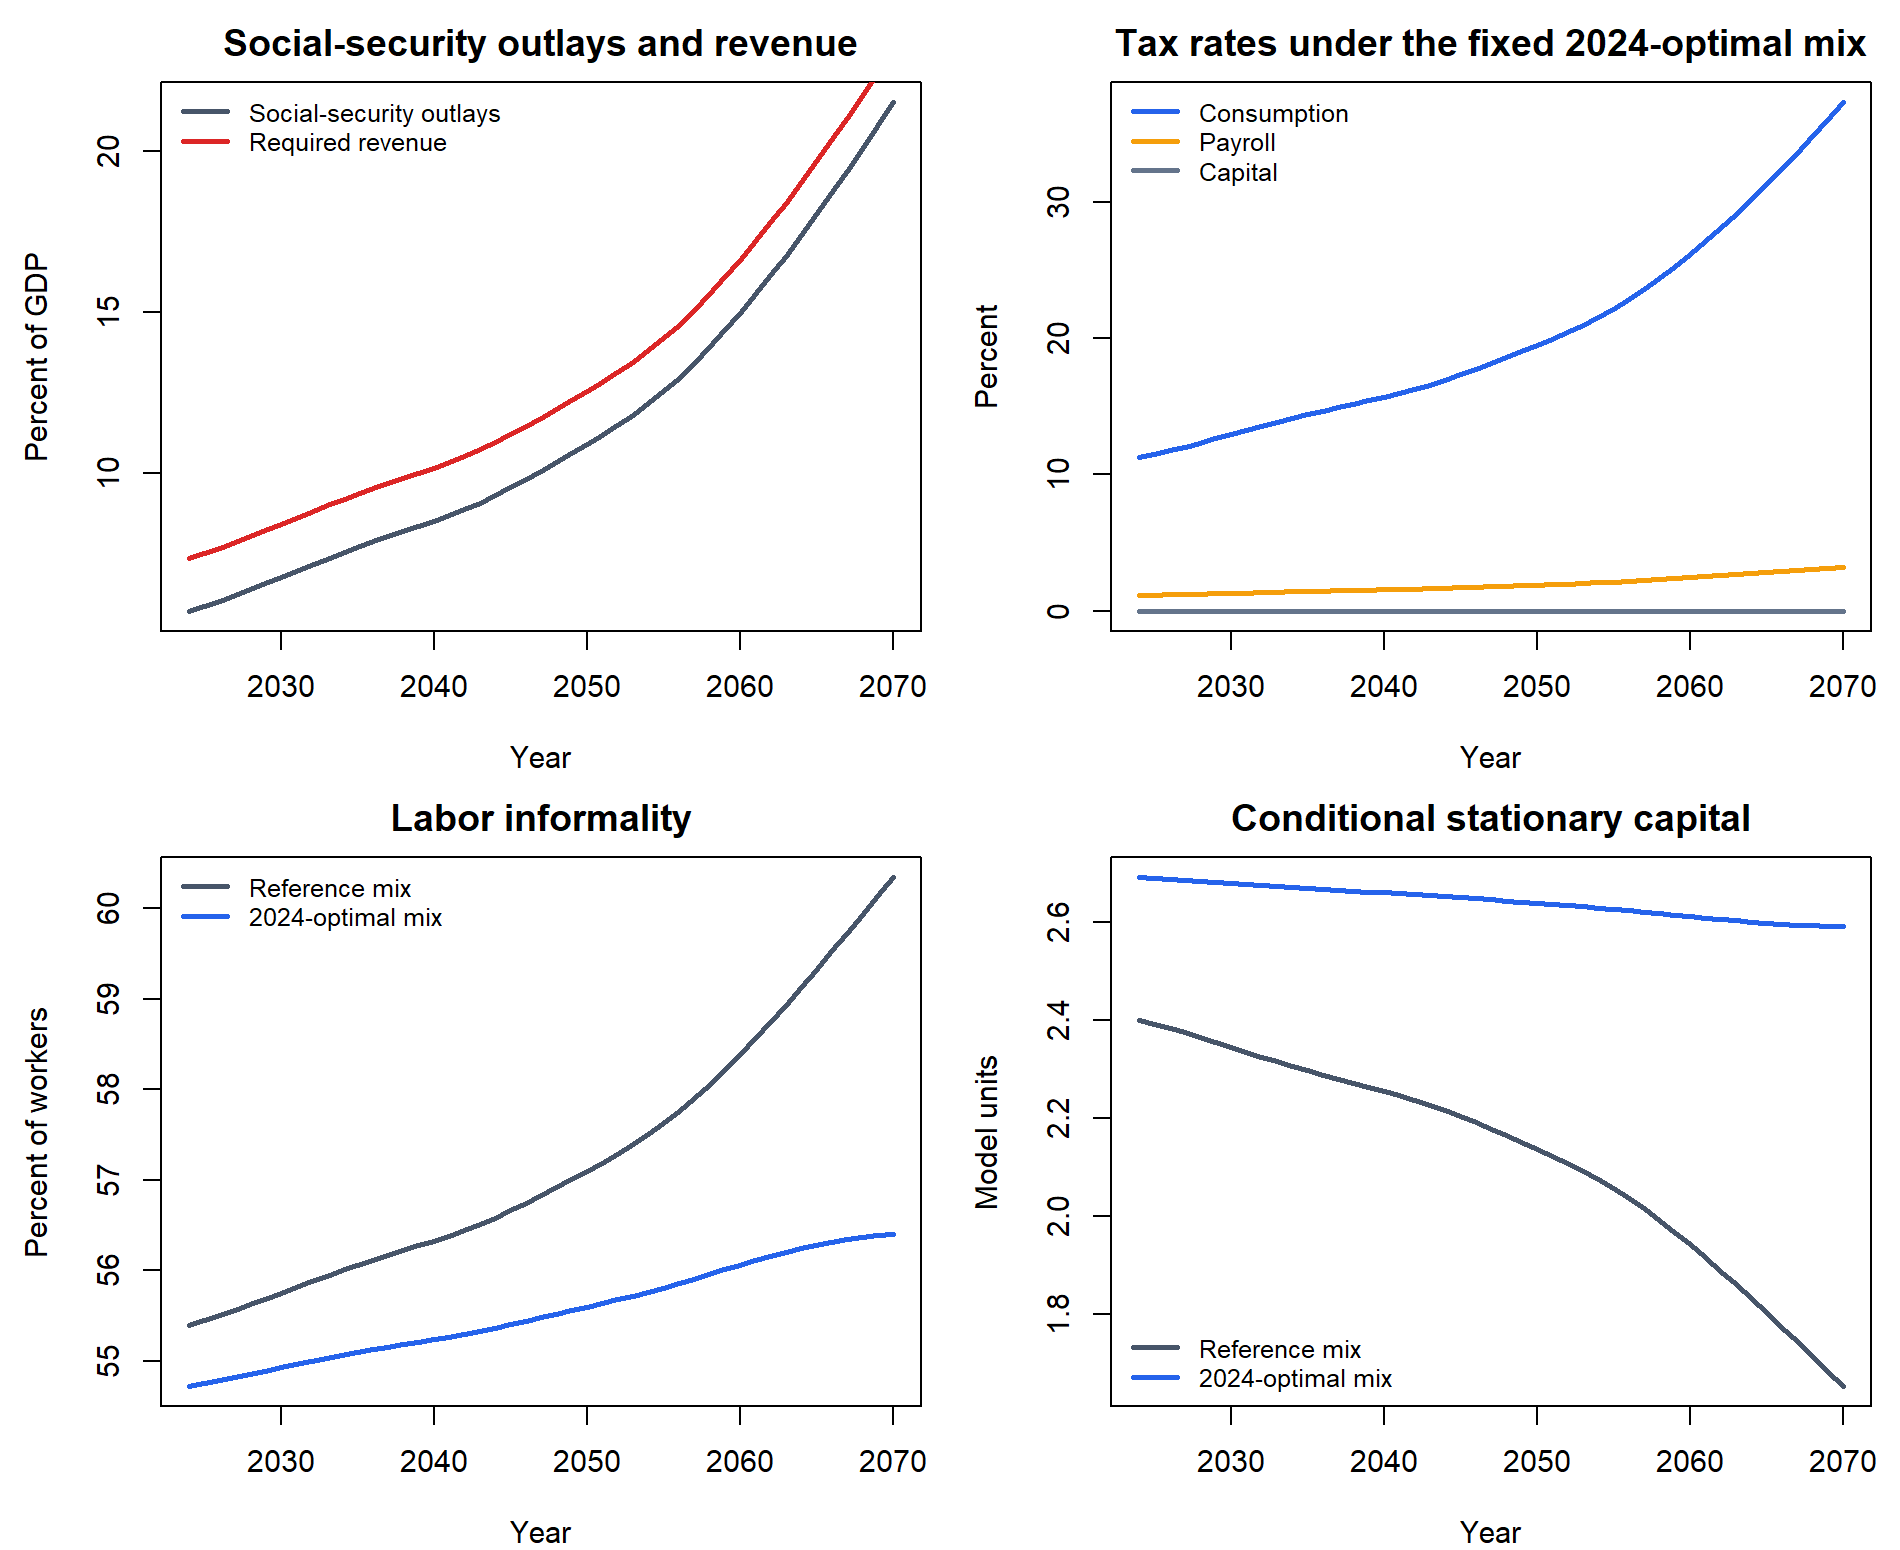
\includegraphics[width=\textwidth]{conditional_aging_paths.png}
\caption{Conditional stationary equilibria along the DANE demographic path}
\label{fig:paths}
\begin{minipage}{0.92\textwidth}
\footnotesize
\emph{Notes:} The reference revenue mix is 45 percent consumption, 35 percent
payroll, and 20 percent capital income. The alternative holds the
2024-optimal shares fixed at 92.5, 7.5, and zero percent. Each annual
observation is a stationary equilibrium conditional on that year's DANE
dependency ratio.
\end{minipage}
\end{figure}

Under the reference mix, informality rises from 55.4 percent in 2024 to 57.1
percent in 2050 and 60.3 percent in 2070. The stationary capital stock falls
from 2.399 to 2.137 and 1.654 model units. Under the fixed 2024-optimal mix,
informality reaches 55.6 percent in 2050 and 56.4 percent in 2070, while
capital remains above 2.59. Composite consumption in 2070 is 0.835 under the
fixed 2024-optimal mix and 0.792 under the reference mix.

The figure does not imply that capital jumps to its next stationary value each
year. It reports how the long-run allocation associated with each demographic
ratio changes. A true transition would impose the predetermined 2024 capital
stock, solve households' intertemporal choices, and let the fiscal rule
determine debt and taxes along one perfect-foresight path.

\subsection{The debt anchor}

Figure \ref{fig:debt} varies $\bar q$ in the 2050 demographic equilibrium and
reoptimizes the tax mix. Raising the anchor from 40 to 70 percent of GDP raises
required revenue from 11.18 to 12.13 percent of GDP. Composite consumption
falls from 0.924 to 0.918, and informality rises from 55.8 to 56.1 percent.
The statutory 55-percent anchor lies between those outcomes.

\begin{figure}[H]
\centering
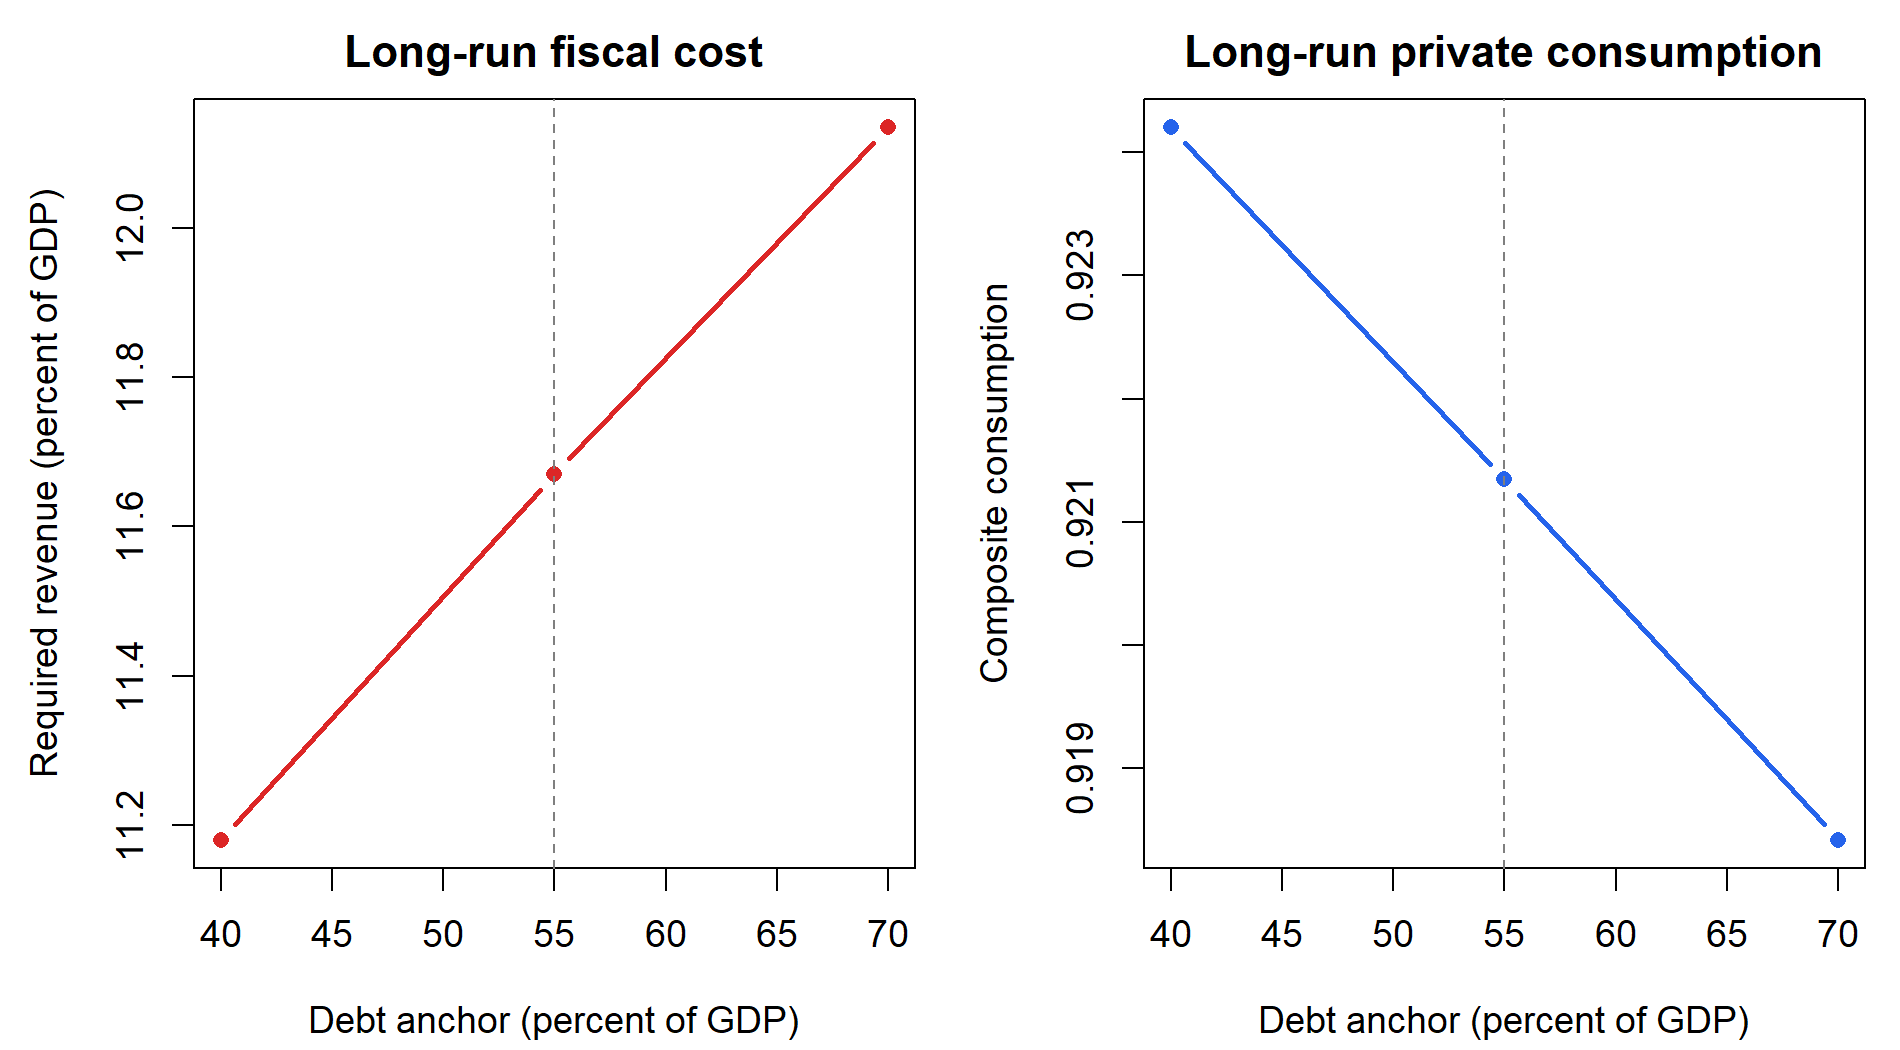
\includegraphics[width=\textwidth]{debt_anchor_2050.png}
\caption{Debt-anchor sensitivity in the 2050 demographic equilibrium}
\label{fig:debt}
\begin{minipage}{0.90\textwidth}
\footnotesize
\emph{Notes:} The dashed line marks Colombia's statutory 55-percent net-debt
anchor. The tax mix is reoptimized at each anchor. The exercise compares
stationary equilibria and does not measure transitional tax smoothing.
\end{minipage}
\end{figure}

A larger $\bar q$ is not a free financing source. At a stationary debt ratio,
the government must raise a primary surplus of
$(r^b-\gamma)\bar q$ to service the debt net of trend growth. A higher anchor
therefore raises long-run taxes and collection costs. Debt can still be useful
during the transition if it prevents tax rates from changing abruptly, as in
the tax-smoothing logic of \citet{Barro1979}. Quantifying that benefit requires
a dynamic transition and cannot be inferred from Figure \ref{fig:debt}.

\section{Limitations and extensions}

The numerical ranking is conditional on six restrictions.

First, the model has one representative dynasty. It contains no
intragenerational variance of consumption and no difference between young and
old households' marginal utilities. The welfare criterion therefore cannot
measure the regressivity of consumption taxes or the distribution of benefits
and tax burdens across generations. Adding household types is necessary
before the paper can answer a distributional version of the research
question.

Second, $\zeta=0.25$ is provisional. Pension payments are transfers, whereas
health and long-term care absorb labor and goods. The aggregate effect of
aging depends on this composition. Administrative records should separately
calibrate cash transfers and real services per older adult.

Third, the collection-cost coefficient is not estimated. The frictionless
comparison shows that it changes the qualitative result from a corner to a
mix. Empirical evidence on compliance, enforcement, and base erosion by
instrument is therefore more important for the tax shares than another digit
of numerical precision in the current grid.

Fourth, the tax rates are reduced-form effective rates. The consumption tax
combines statutory rates, exemptions, and incomplete informal coverage. The
payroll tax combines mandatory contributions and other formal-employment
costs. The capital tax does not distinguish normal returns from rents. Direct
comparison with Colombian statutory rates would be misleading.

Fifth, the annual paths are conditional stationary equilibria. They do not
contain capital and debt transition dynamics, unexpected demographic news, or
cohort-specific saving. The next version should solve the perfect-foresight
path with $K_{2024}$ and $B_{2024}$ predetermined.

Sixth, $\bar q$ is a policy parameter rather than an optimized state. An
endogenous debt anchor requires a sovereign-risk premium, an explicit
probability of fiscal stress, or an external-debt margin. Without one of those
costs, the transition benefit of borrowing is not identified separately from
the stationary interest bill.

\section{Conclusions}

Population aging converts a fixed real outlay per older adult into a rising
revenue requirement per working-age adult. DANE's projected dependency ratio
almost doubles between 2024 and 2050 and exceeds 48 percent by 2070. The
government's financing choice therefore changes the long-run allocation even
when the benefit received by each older adult remains constant.

In the benchmark model, the stationary tax mix relies primarily on
consumption and secondarily on formal payroll. The payroll share rises as the
population ages because convex collection costs make it increasingly costly
to concentrate the entire revenue requirement in consumption. The
capital-income share is zero because capital accumulation is elastic and the
representative household removes distributional motives for capital taxation.

Two negative results are equally important. Imperfect substitution between
formal and informal consumption does not by itself prevent a corner solution:
without collection costs, the model finances everything through consumption.
Public debt also does not remove the permanent tax requirement. A higher debt
anchor raises stationary interest payments and lowers consumption.

The current results establish a mechanism, not a Colombian tax package. The
next empirical step is to estimate the collection and base-erosion costs of
each instrument. The next modeling step is to add heterogeneous young and old
households and solve the full transition. Those additions would allow the
paper to compare efficiency, intragenerational incidence, and
intergenerational welfare within the same policy experiment.

\appendix
\section{Numerical algorithm}

The replication uses base R and proceeds in six steps.

\paragraph{1. Demographic input.}
The script reads annual DANE populations aged 15--64 and 65 and over for
2024--2070. It constructs $d_t=N_t^o/N_t^y$ without interpolation.

\paragraph{2. Calibration.}
At the 2024 dependency ratio, the code chooses
$(\bar g_o,\kappa)$ to minimize the squared distance from the 5.7-percent
spending target and 55.4-percent informality target under the reference
revenue mix. The outer problem uses Nelder--Mead.

\paragraph{3. Stationary equilibrium.}
For a given $(d,\boldsymbol{\omega},\bar q)$, the unknown vector is
\[
 z=\left(\log K,\operatorname{logit}L^F,\log p^I,\log C^F\right).
\]
The transformations impose $K>0$, $p^I>0$, $C^F>0$, and
$L^F\in(0,1)$. From $z$, the code computes production, factor prices,
social-security spending, required revenue, tax bases, tax rates, and
collection costs.

The four residuals are the formal-labor choice
\eqref{eq:formal_choice}, CES relative demand \eqref{eq:relative_demand},
capital Euler condition \eqref{eq:euler}, and formal-goods market
\eqref{eq:formal_market}. BFGS minimizes the sum of squared residuals.
Four dispersed starting values are used for a standalone solution. Adjacent
tax mixes use the preceding equilibrium as a warm start. Nelder--Mead is a
fallback when the residual norm remains above tolerance.

\paragraph{4. Policy search.}
The code first evaluates a simplex grid with increments of 0.10. It then
evaluates a local grid with increments of 0.025 around the best coarse point.
The reported optimum is the feasible point with the highest stationary
utility. The procedure does not impose positive shares.

\paragraph{5. Counterfactuals.}
The tax mix is optimized at the 2024, 2050, and 2070 dependency ratios. The
2050 problem is repeated for debt anchors of 40, 55, and 70 percent. The
frictionless counterfactual sets every $\chi_j$ to zero. Annual conditional
paths hold either the reference mix or the 2024-optimal mix fixed.

\paragraph{6. Verification.}
Automated tests require the calibrated equilibrium to match both targets,
each equilibrium residual to be below tolerance, tax rates to be
nonnegative, the policy grid to contain one optimum, and social-security
spending as a share of output to rise across selected demographic years.
All figures and LaTeX macros are generated from the same result files used in
the text.

\bibliographystyle{apalike}
\bibliography{references}

\end{document}
